% This version of CVPR template is provided by Ming-Ming Cheng.
% Please leave an issue if you found a bug:
% https://github.com/MCG-NKU/CVPR_Template.

%\documentclass[review]{cvpr}
\documentclass[final]{cvpr}
\usepackage{times}
\usepackage{epsfig}
\usepackage{graphicx}
\usepackage{amsmath}
\usepackage{amssymb}
\usepackage{svg}
\usepackage{subfig}
\usepackage[printonlyused, smaller]{acronym}
\usepackage{multirow}
\usepackage{makecell}
% Include other packages here, before hyperref.
\usepackage{algorithm}
\usepackage{algpseudocode}

% If you comment hyperref and then uncomment it, you should delete
% egpaper.aux before re-running latex.  (Or just hit 'q' on the first latex
% run, let it finish, and you should be clear).
\usepackage[pagebackref=true,breaklinks=true,colorlinks,bookmarks=false]{hyperref}


\def\cvprPaperID{****} % *** Enter the CVPR Paper ID here
\def\confYear{CVPR 2022}
%\setcounter{page}{4321} % For final version only


\begin{document}

%%%%%%%%% TITLE
\title{Camera Pose Estimation using Regression Forest and RANSAC Optimization}

\author{Falk Ebert\\
\tt 4018276\\
{\tt\small falk.ebert@stud.uni-heidelberg.de}
% For a paper whose authors are all at the same institution,
% omit the following lines up until the closing ``}''.
% Additional authors and addresses can be added with ``\and'',
% just like the second author.
% To save space, use either the email address or home page, not both
\and
Jason Pyanowski\\
\tt 3663907\\
{\tt\small jason.pyanowski@stud.uni-heidelberg.de}
\and
Marven Hinze\\
\tt 3664283\\
{\tt\small marven.hinze@stud.uni-heidelberg.de}
\and
Nadine Theisen\\
\tt 3475402\\
{\tt\small nadine.theisen@stud.uni-heidelberg.de}
}

\maketitle


%%%%%%%%% ABSTRACT
\begin{abstract}
This project aims to realize the approach of~\cite{shotton2013} to infer the position and rotation of a camera
in the 3D world space given a set of 2D images. A regression forest is used to predict the correspondencies between 
pixels and world coordinates using RGB and depth information. An initial set of hypothesized camera
poses are deduced by applying the regression forest and are then optimized with a preemptive RANSAC. The algorithm 
is evaluated on the 7-scenes dataset~\cite{glocker2013} which contains RGB images with corresponding depth
information for each pixel of 7 different 3D scenes. Subsequently, the ability of the forest to predict 2D-3D 
correspondencies is evaluated. To verify the estimated camera poses of the RANSAC algorithm, the translational and 
angular error with respect to the known ground truths are measured. These findings are then compared to the results
of~\cite{shotton2013}. 
\end{abstract}

%%%%%%%%% BODY TEXT
\section{Introduction}

In this project, we provide an approach of interferring the pose of a camera in the world coordinate system. 
Given a data set consisting of RGB-D images as well as camera pose matrices, the camera for a given frame can 
be localized. The method we use is based on the paper by \cite{shotton2013}.  The whole process is divided into 
two subsequent steps which will be explained in more detail in the following sections.
\begin{enumerate}
\item Finding correspondencies between 2D image pixels and 3D world coordinates  \\

In the first step, we apply a \textit{Regression Forest} to a perform scene coordinate regression. 
A regression tree can be evaluated at any 2D image pixel \textbf{p} and predicts the corresponding position 
in the 3D world space of the scene as a combination of the predictions of all decision trees in the forest. 
We use the scene coordinates introduced by \cite{shotton2013} as labels for training the regression forest. 
Using the calibrated depth \textit{D}(\textbf{p}), it is possible to compute the 3D camera space coordinate 
textbf{x} which can be transformed into the scene's world coordinate frame with the camera pose matrices \textit{H}
 giving  the scene world coordinates \textbf{m}. The forest is then trained on randomly chosen sets (\textbf{p,m})
  for each tree.

\item Optimizing the camera pose for a given image \\
In this part, the scene coordinates associated with a 2D pixel will be used to estimate the camera location and
 orientation. The location is estimated by minimizing an energy function over a camera pose hypothesis \textit{H} 
 determined by applying the regression forest on a small set of pixels. Then, the number of pixels which are 
 outliers according to the included error function is counted. The energy is optimized using a RANSAC algorithm.
  In the first step, the energy of a set of initial hypotheses is updated after evaluating the forest at a random 
  sample of pixels.
\end{enumerate}
    
    

% What are we doing in this project?
%	-> Scene coordinate regression
% 	-> Camera pose estimation
% Why is this important?

% What data is given
% 	-> Image data including depth, camera poses
We use the 7-scenes dataset~\cite{glocker2013} set which consists of seven different scenes with each between 
2,000 and 12,000 frames. To each frame the corresponding depth map and the 4×4 matrix \textit{H} in homogeneous 
coordinates which encodes the rotation and the translation from camera space to world space. The full data set 
was obtained using a Kinect RGB-D camera at 640×480 resolution. The dataset is split into training and test data.

%-------------------------------------------------------------------------
\subsection{Related Work}
Nowdays, many approaches to infer camera poses or poses of objects in general are based on either image-based approaches or 
sparse keypoint matching. The application of imaged-based pose estimation uses the whole image and matches different frames 
using high level features like \ac{SIFT} or \ac{SURF}~\cite{Klein2008}. Thereby, an initial camera pose is refined using 
the obtained features and known camera poses. The result is then calculated as a weighted average over the 
images that describe the camera pose best. 

More recently, approaches concerning sparse feature matching gained interest~\cite{Holzer2012}. Again, high level features are detected but 
instead matched with a large set of feature descriptors. This approach requires a lot of engineering regarding the feature
description and matching process. The routine of inferring a camera pose presented in the reference paper of Shotton et al.~\cite{shotton2013}
comes the difference that only low-level features are utilized. Simple pixel-based features are applied in order to train a
regression forest without the need of feature descripters. The predictions of the camera pose are then made directly one the
output of the forest which correlates 3D image pixels with 3D world coordinates. The underlying forest can additionally be 
evaluated for abritrary pixel positions and is therefore sparse.


\section{Methods}
%-------------------------------------------------------------------------
This section gives an overview of the methods used in this project. We will discuss
the concept of regression forests including feature extraction and the RANSAC algorithm
used for estimating the camera pose from the image data. We will not discuss all aspects
in full detail but only provide further explanations where we find it relevant
for the presentation of our work and results.

\subsection{Data Preperation}
%-------------------------------------------------------------------------
To train the regression forest the 7-scenes datset~\cite{glocker2013} is utilized. 
Each scene consists of multiple image sequences that cover the are of interest. Using a RGB-D 
Kinect camera, depth information for each pixel is extracted. The resolution of the $24$ 
bit RGB-images is $640\times480$ pixels and the corresponding $16$ bit depth map is given 
in millimeters. For each image a $4\times4$ ground truth camera pose in homogenous coordinates 
is provided, which allows to validate the estimated camera pose matrix for a given image. 
Each dataset is split randomly into train and test. 

Based on that, our data set is composed of a number of samples $\{(\boldsymbol{p}_i, \boldsymbol{w}_i)\}$ with
$\boldsymbol{p}_i = (x_l, y_l)_i$ and $\boldsymbol{w}_i = (x_s, y_s, z_s)_i$ where the subscripts
$l$ and $s$ denote image pixel coordinates and scene coordinates respectively.\\

\subsection{Regression Forest}
%-------------------------------------------------------------------------

In this project we use a regression forest to predict scene coordinates for a given
sample image coordinate as suggested in \cite{shotton2013}. In this section we will
give some background on the concept of regression forests, the pixel coordinate
labeling and the image-feature extraction on which the forests base their predictions.\\

\subsubsection{Decision Trees}
%-------------------------------------------------------------------------
A regression forest consists of a number $N$ of regression trees, which each consist of
of root node and it's children~\cite{Criminisi2013}. We consider the special case of binary decision trees
where each node (unless it is a leaf node) has a left and a right child. Each node $n$
stores a set of parameters $\theta_n$ which are used in the calculation of a
feature response function $f_{\theta}(\boldsymbol{p}) \in \{1, 0\}$ which determines if the input
data point $\boldsymbol{p}$ is branched to the left or right child node. To every leaf node
(i.e. a node without children) we assign a response value $\boldsymbol{w}_n$ representing
the tree's prediction for a data point $\boldsymbol{p}$ that has reached this node. In our
specific application the input data points $\boldsymbol{p}$ are 2D pixel coordinates and the
responses $\boldsymbol{w}$ are 3D world coordinates.

The process of training the tree involves finding the set of parameters
$\{\theta_n | \, \forall \, \text{nodes} \, n\}$ which results in the best predictions
for previously unseen input data points $\boldsymbol{p}$. However, this final goal cannot
be optimized directly during training, as this would entail optimization in the
very large space of all possible parameters for all tree-nodes simultaneously. Therefore
it is much more efficient to optimize the parameters one node at a time using a
proxy-objective $Q(S_{\text{tot}},\, S_{\text{left}}(\theta),\, S_{\text{right}}(\theta))$
which ideally leads to a similar result.

Let $S_{\text{tot},n} = \{ (\boldsymbol{p}_i, \boldsymbol{w}_i) \, | \, i \in |S_n|\}$ denote the
input data and target response for a given node $n$. According to its parameters the
node splits this set into the subsets
\begin{equation}
\begin{split}
	S_{\text{left},n}(\theta_n) = \{(\boldsymbol{p}_i, \boldsymbol{w}_i) \,|\, f_{\theta_n}(\boldsymbol{p}_i) = 0\} \\
	S_{\text{right},n}(\theta_n) = \{(\boldsymbol{p}_i, \boldsymbol{w}_i) \,|\, f_{\theta_n}(\boldsymbol{p}_i) = 1\}
\end{split}
\end{equation}
corresponding to left and right child node respectively. The objective function $Q$ is
then used to assign a score to the split resulting from the parameters $\theta_n$ at
this node.

The objective function used here optimizes for a reduction in variance of the target 
responses (i.e. "wants the tree to group together points with similar scene coordinates").
Defining $W_n = \{ \boldsymbol{w}_i \, | \, (\boldsymbol{p}_i, \boldsymbol{w}_i) \in S_n \}$ this
objective can be mathematically expressed as:
\begin{multline}
	Q(W_\text{tot}, \theta) =
		\text{Var}(W_\text{tot})\, - \sum_{d\,\in\{\text{left,\,right}\}}
			\dfrac{|W_d(\theta)|}{|W_\text{tot}|} \text{Var}(W_d(\theta))\\
	\text{with} \hspace{5mm} \text{Var}(W) = |W|^{-1} \sum_{\boldsymbol{w}\in W} ||\boldsymbol{w} - \bar{\boldsymbol{w}}||_2^2
\end{multline}
Training the complete tree then involves choosing a set of images from which a number
of sample pixels is drawn. These samples are then evaluated (i.e. split into left and right set)
by the tree's root node for a number of parameter-sets. For each set of parameters, the
split's score is calulacted using the objective function and the optimal parameters for
this node are recorded. The process is then repeated for the node's children with the corresponding
set (left or right; split according to the optimal parameters) until either the set contains
only one element or the maximum depth is reached.
When the maximum depth is reached and the set still contains more than one element, a response
needs to be calculated for the node. This response represents the tree's prediction for 
all pixels, which reach this node and is calculated from the sample's ground truth scene coordinates.
In practice, a mean shift variance algorithm \cite{Comaniciu2002} is used to find the center of the 
largest cluster. Thereby, at most $500$ random coordinates are utilized for calculation to limit 
the computational cost.

\subsubsection{Image Features}
%-------------------------------------------------------------------------
In order to use a decision tree to infer scene coordinates from the pixel coordinates,
it is necessary to calculate features associated with a given pixel coordinate from the
image data. This is implemented in the feature response function mentioned earlier.
We have chosen to use the 'Depth-Adaptive RGB' image features from \cite{shotton2013} which
is defined as
\begin{equation}
	f_{\theta}^{da-rgb}(\boldsymbol{p}) = I\left(\boldsymbol{p} + \frac{\boldsymbol{\delta}_1}{D(\boldsymbol{p})}, c_1\right)
	- I\left(\boldsymbol{p} + \frac{\boldsymbol{\delta}_2}{D(\boldsymbol{p})}, c_2\right)
\end{equation}
where $I(\boldsymbol{p}, c)$ is the images value in the $c \in \{\text{r, g, b}\}$ component at
the pixel location $\boldsymbol{p}$ and the 'Depth' image feature specified as
\begin{equation}
	f_{\theta}^{depth}(\boldsymbol{p}) = D\left(\boldsymbol{p} + \frac{\boldsymbol{\delta}_1}{D(\boldsymbol{p})}\right)
	- D\left(\boldsymbol{p} + \frac{\boldsymbol{\delta}_2}{D(\boldsymbol{p})}\right)
\end{equation}
where $D(\boldsymbol{p})$ refers to the depth value corresponding to pixel $\boldsymbol{p}$.
The parameters are given explicitly as $\theta = \{\boldsymbol{\delta}_{1,2}, c_{1,2}, \tau\}$. 
The offsets $\boldsymbol{\delta}_{1,2}$
allow the tree node to incorporate non-local information for each pixel. When the resulting
lookup location is outside the image boundary, the original sample pixel $\boldsymbol{p}$ is
disregarded in training and can also not be predicted by the forest. The parameter threshold 
$\tau$ is used to decide if the feature is split to the right or left child node according to 
$f_{\theta}(\boldsymbol{p}) \leq \tau$.


%-------------------------------------------------------------------------
\subsection{RANSAC Optimization}
The predicted world scene coordinates of the forest are used to derive the corresponding camera pose matrix for a given image. 
The objective of the optimization is to find a camera pose matrix that minimizes an energy $E$,
\begin{equation}\label{energy_function}
	E(H) = \sum_{i \in I} \rho(\min_{\boldsymbol{m} \in \boldsymbol{M_{i}}} 
	\| \boldsymbol{m} - H \boldsymbol{x_{i}} \|_{2}) = \sum_{i \in I}e_{i}(H)
\end{equation}
where as $i \in I$ is a pixel index,  $\rho$ a top-hat error function with a width of $0.1$m, $M_{i}$ 
the set of predictions for pixel $\boldsymbol{p_{i}}$, $H$ a camera pose hypothesis and $\boldsymbol{x_{i}}$ is the camera
scene coordinate of $\boldsymbol{p_{i}}$ \cite{shotton2013}. If $\rho$ returns $0$ for a given pixel, it is considered
to be an inlier, otherwise it is an outlier.

The hypotheses optimization is based on an adapted version of preemptive RANSAC \cite{shotton2013}.
Algorithm \autoref{ransac} shows the pseudo-code of the RANSAC optimization.
The procedure starts with the initialization of $K$ hypotheses for the camera pose matrix. 
The next step is to create a pixel batch $B$,
each hypothesis is evaluated on this batch. The resulting inliers per hypothesis  are stored and their energy is 
updated. Furthermore, to reduce the runtime, the mode $\boldsymbol{m}$ from \ref{energy_function} is stored for
the pixel inlier.
The next step is to sort the hypotheses by their energy in ascending order and discard the top half. Next, the remaining hypotheses are refined.

\begin{algorithm}
	\caption{RANSAC optimization}\label{ransac}
\begin{algorithmic}[1]
	\State  $K \gets K_{init}$
	\State initialize hypotheses $\{ H_{K} \}_{k=1}^{K}	$
	\State initialize energies $E_{k}$
	\While{$K > 1$}
		\State sample random pixel batch $B$
		\ForAll{$i \in B$}
			\State $\boldsymbol{M_{i}} = forest(i)$
			\ForAll{$k \in \{1, ..., K\}}$
				\State $E_{k} \gets E_{k} + e_{i}(H_{k})$
				\If{$e_{i}(H_{k})$ is $0$}
					\State add i to $inliers_{k}$
					\State add $\boldsymbol{m}$ to $modes_{k}$
				\EndIf
			\EndFor
		\EndFor
		\State sort hypotheses by $E_{k}$
		\State $K \gets \lfloor \frac{K}{2} \rfloor$
		\State refine hypotheses $H_{k}$ on $inliers_{k}$ for $k=1, ...,K$

	\EndWhile
	
	\State \Return $H_{k}$
	
\end{algorithmic}
\end{algorithm}

\subsubsection{Hypotheses initialization}
To initialize a hypothesis, three random pixels $\boldsymbol{p_{i}}$ with $i \in \{0,1,2\}$ are sampled. The pixel $\boldsymbol{p_{i}}$ must have a depth unequal to $6553$ and $0$. Every $\boldsymbol{p_{i}}$ is evaluated on the forest, this results in three sets 
$\boldsymbol{M_{i}}$ containing the prediction $\boldsymbol{m}$ from every tree. For each $p_{i}$ a random prediction is sampled from $\boldsymbol{M_{i}}$. Furthermore, for every $\boldsymbol{p_{i}}$ the camera scene coordinate $\boldsymbol{P}$ is calculated.

\begin{equation}
	\boldsymbol{P} = (\boldsymbol{C}^{-1} \cdot \boldsymbol{\tilde{p_{i}}} ) \cdot d
\end{equation}

where $\boldsymbol{C}$ is the intrinsic camera matrix, $\boldsymbol{\tilde{p_{i}}}$ the pixel $\boldsymbol{p_{i}}$ in
homogeneous coordinates and $d$ is the depth value for $\boldsymbol{p_{i}}$ in meters. 

For finding the best
rotation between the camera scene and world coordinates, the Kabsch algorithm is used. The Kabsch algorithm allows to find the best rotation that transforms one set of vectors into a second set of vectors \cite{Kabsch1976}.
Let $M$ be a matrix containing the camera scene coordinates row wise and $W$ a matrix containing
the world coordinates, where as $\boldsymbol{\bar{m}}$ and $\boldsymbol{\bar{w}}$ are the mean coordinates.
To find the best rotation one needs to compute the cross covariance matrix $C$ of $M$ and $W$, the 
next step is the application of a singular value decomposition on $C$ \cite{Brachmann2020}.

\begin{equation}
	C = U \Sigma V^T
\end{equation}

The optimal rotation $R$ and the translation $\boldsymbol{t}$ are then obtained by \cite{Brachmann2020}:

\begin{equation}
	\begin{split}
		R &= V 
		\begin{bmatrix}
			1 & 0 & 0\\
			0 & 1 & 0\\
			0 & 0 & det(VU^T)
		\end{bmatrix}
		U^T \\
		\boldsymbol{t} &= \boldsymbol{\bar{w}} - R \boldsymbol{\bar{m}}
	\end{split}
\end{equation}
 By combining $R$ and $\boldsymbol{t}$ into an affine transformation the initial hypothesis $H$ is obtained.
 
\subsubsection{Pose refinement}
For refinement of a hypothesis the respective pixel inliers are retrieved and their camera scene 
coordinates are calculated. These camera scene coordinates and the stored predictions for the pixel inliers 
are passed to the Kabsch algorithm, the returned affine transformation is then considered as the refined pose.



%-------------------------------------------------------------------------
\section{Experiment Evaluation} \label{sec:eval}
To verify the outcome of the regression forest and consecutive RANSAC optimization, the utilized metrics are described
in the following section. As basic error measurement of the forests predicted world coordinates to the ground truth the 
$\ell^2$-norm us used. Thereby, the error per scene is calculated by taking the average deviation in meters 
over all trees within a forest. 

The camera poses predicted by the RANSAC algorithm are compared using the translational and angular error 
which are further described in the subsection below. All findings are then related to the results obtained by 
Shotton et al.~\cite{shotton2013}. 


\subsection{Metrics} \label{subsec:metrics}
To evaluate the estimated camera poses, the translational and angular error with respect to the 
ground truth camera poses is measured. Let the estimated pose matrix $H_{est}$ and the ground truth 
$H_{gt}$ be $4 \times 4$ matrices
in homogeneous coordinates that encode the location and orientation of the camera in the world 
coordinate system. To measure the translational offset between them, the translation vectors 
$\boldsymbol{t_{est}}, \boldsymbol{t_{gt}} \in \mathbb{R}^3$ of the matrices are used.
By applying the $\ell^2$-norm to the translation vectors, the translational error is obtained by
\begin{align}
    \varepsilon_t &= \sqrt{\sum_{x,y,z}||\boldsymbol{t_{est}} - \boldsymbol{t_{est}}||^2}.
\end{align}
To compare two rotational poses, the angle of the difference rotation matrix $R$ is utilized. 
Denote the whole $3\times3$ upper-left matrix of $H_{est}$ and $H_{gt}$ as $R_{est}$ and 
$R_{gt}$ repectively. They refer to the orientation in space and the difference rotation can be computed 
as $R = R_{est}^TR_{gt}$. The angle between those two rotation matrices is the desired
error measure and defined as
\begin{align}
    \varepsilon_r &= arccos \left( \frac{tr(R)-1}{2} \right)
\end{align}
where $tr(R)$ is the trace of a matrix.

% \subsection{??}
% das vllt in die einleitung und ein chapter für die metrics vom tree 

%-------------------------------------------------------------------------
\section{Results}
In this section we give some background on the implementation and the parameters that have been chosen in order to 
run the forest and RANSAC optimization. Then, the findings are evaluated according to the measurements described
in Section~\ref{sec:eval}. Firstly, it is investigated how accurate the 
forest predicts the 3D world coordinates from 2D image coordinates. Subsequently, the trained forest is used to obtain 
the camera poses for a number of unseen test images using RANSAC optimization. Four out of the seven scenes 
are evaluated and their results are compared among them and to the reference paper of Shotton et al.~\cite{shotton2013}. 

\begin{table}[h!]
	\begin{center}
	\begin{tabular}{|l|c|}
	\hline
	Hyperparameter & Value \\
	\hline\hline
	Number of Trees & $5$ \\
	Max Tree Depth & $16$ \\
	Batch Size & $500$ \\
	Pixel Samples per Image & $5000$ \\
	Parameter Samples per Image  & $1024$ \\
	Feature Type & DA-RGB \\
	\hline
	\end{tabular}
	\end{center}
	\caption{Hyperparameters used for training forests.}
	\label{tab:params-forest}
\end{table}

\subsection{Implementation and Parameter Settings}
For the scenes \textit{Chess}, \textit{Fire},  \textit{Pumpkin},  \textit{Red Kitchen} and  \textit{Stairs} a forest is
trained. These scenes are chosen because they show the most significant results for the feature type 'Depth Adaptive RGB' 
which is considered for the following evaluations.

The forests are trained with the hyperparameters given in Table~\ref{tab:params-forest} and are chosen according to the 
values given in~\cite{shotton2013}. The number of parameter samples per image wasn't given and we found the
value $1024$ to work out well, because further increase wasn't improving the number of correct world coordinate predictions.

\begin{table}[h!]
	\begin{center}
	\begin{tabular}{|l|c|}
	\hline
	Hyperparameter & Value \\
	\hline\hline
	Size of batch $B$ & $500$ \\
	$K_{init}$ & $1024$ \\
	
	\hline
	\end{tabular}
	\end{center}
	\label{tab:params-ransac}
	\caption{Hyperparameters used RANSAC optimization.}
\end{table}

The consecutive RANSAC optimazation uses the parameters given in~\ref{tab:params-ransac}. 


Finally, for each scene a total of $500$ random images from the test data with each having $5,000$ test pixels are used
to predict the corresponding camera poses. 

\textbf{Runtime}: is ...

%At first, each trained forest (per scene) is analyzed in 
%terms of the ability to find 2D-3D correspondencies. Then, the estimated camera poses are evaluated as described 
%in~\ref{subsec:labels} and compared to the findings in~\cite{shotton2013}.


\subsection{Image to World Point Correspondencies}
The forests exhibits the basic ability to predict 3D world coordinates based on 2D image pixels and 
qualitative results are shown in~\ref{fig:pointclouds}. For each scene, the regression forest is evaluated by 
randomly choosing $500$ images and sampling $5,000$ pixels from the test data set. The pointclouds 
allow to recognize the scenes even by a sparse number of utilized sample pixels. 

However, most scenes show areas where no 3D coordinates
were predicted. This could be attributed to a false prediction of 3D points. Due to the fact that the forest is 
trained on known world coordinates, the assignment of a pixel to a world point that is actually present in the 
scene is possible. 

\begin{figure}[h!]
	\begin{center}
	
	\subfloat[~Chess]{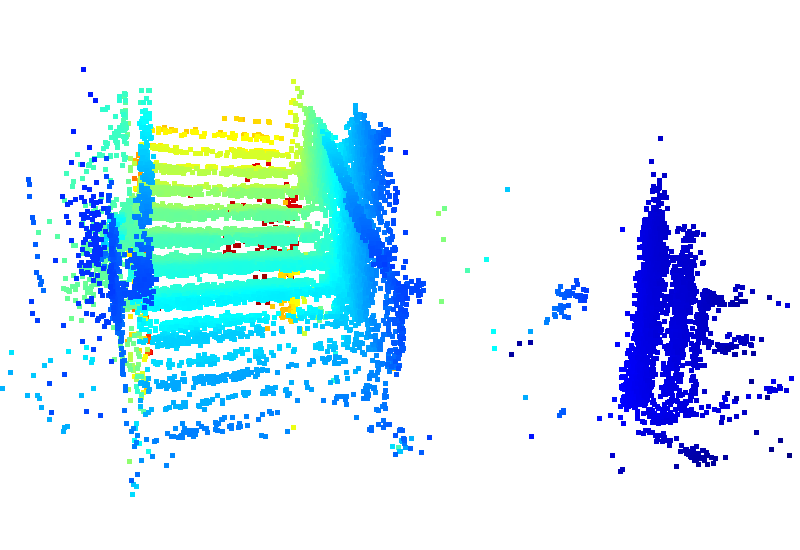
\includegraphics[width=0.2\textwidth]{images/pcs_stairs.png}}\,
	\subfloat[~Fire]{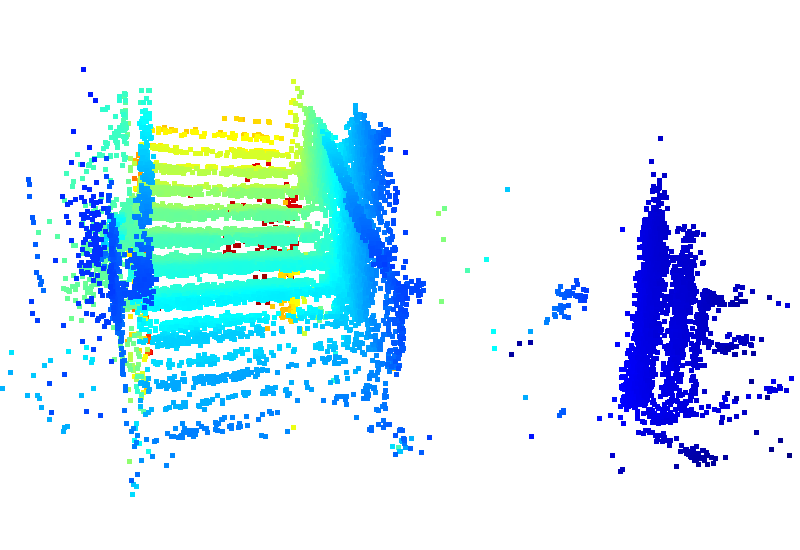
\includegraphics[width=0.2\textwidth]{images/pcs_stairs.png}}\,
	\\
	\subfloat[~Pumpkin]{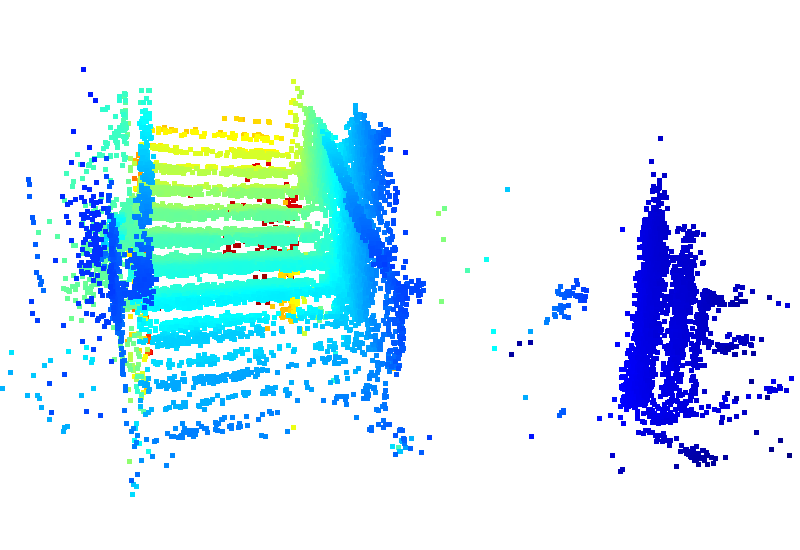
\includegraphics[width=0.2\textwidth]{images/pcs_stairs.png}}\,
	\subfloat[~Red Kitchen]{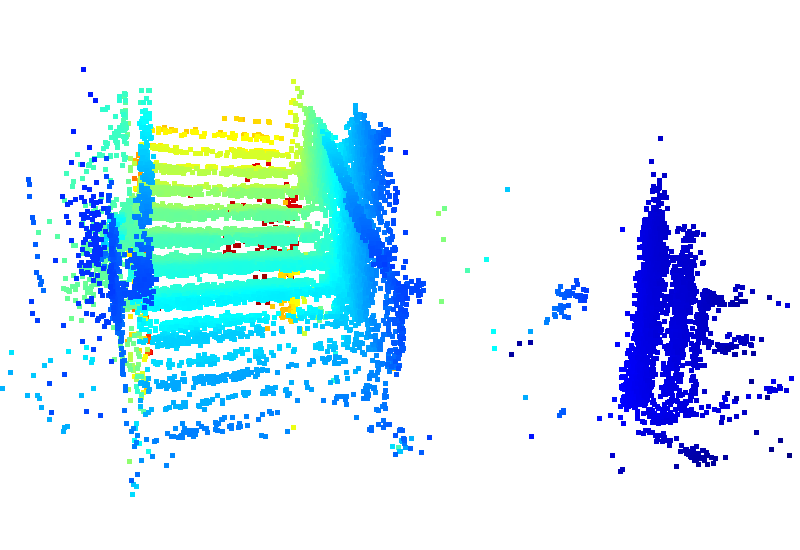
\includegraphics[width=0.2\textwidth]{images/pcs_stairs.png}}\,
	\subfloat[~Stairs]{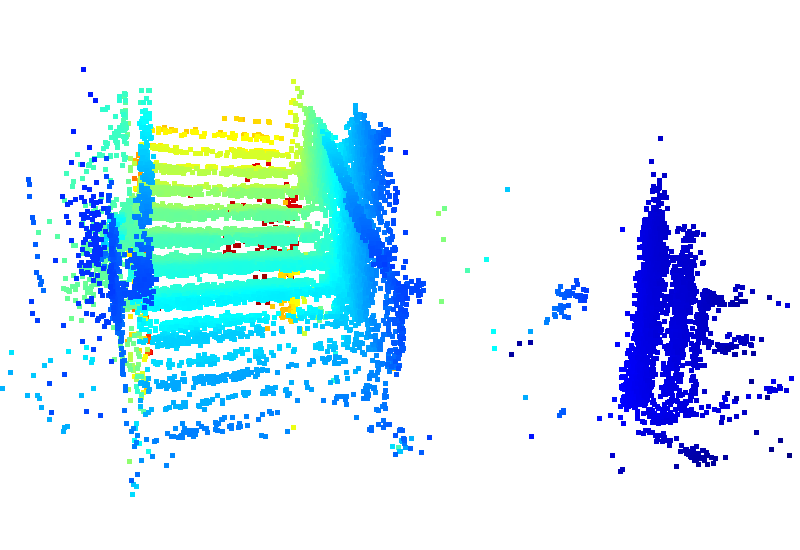
\includegraphics[width=0.2\textwidth]{images/pcs_stairs.png}}

	\end{center}
	\caption{For each scene a forest is trained with the hyperparameters stated in~\ref{XX}. The forest 
	is then evaluated for $500$ test images with each having $5,000$ sample pixels. For each pixel the coresponding
	3D world coordinate is obtained. The resulting pointclouds are displayed in subfigures (a)-(g). }
	\label{fig:pointclouds}
	\label{fig:onecol}
\end{figure}

Another explanation are invalid values during feature generation. Correspondencies that could not be predicted are
caused by the fact that sample pixels are potentially shifted out of the image frame or correspond to an invalid depth value. 
Predicting the 3D world coordinates for all scenes, the forests exhibit $91.2\%$ valid predictions on average. 
This implies that a forest is capable of finding correspondencies.

To further investigate these findings, the predicted coordinates of the forest are compared to the known ground truths using 
the $\ell^2$-norm. In Table~\ref{tab:forest-error} the deviation in meters and corresponding variance indicates rather large 
errors. It varies among $x.y$m for the scene XY to $x.y$m for the scene CSAS. This suggests that the mapping is not as precise
as desired. By looking at the histogram of accumulative errors for each scene in Figure~\ref{fig:error-hist}, it appears that 
there exist numerous predictions with small error. It can therefore be expected that the poses that will be predicted by the 
RANSAC algorithm still produce desirable results due to its greedy approach.  

\begin{table}
	\begin{center}
	\begin{tabular}{|l|c|}
	\hline
	Scene & average deviation [m]\\
	\hline\hline
	Chess 		& 	$1.079 \pm 0.388$ \\
	Fire 		& 	$0.893 \pm 0.313$	\\
	Heads 		& 	$0.0 \pm 0.0$	\\
	Office 		&   $0.0 \pm 0.0$ \\
	Pumpkin 	& 	$1.413 \pm 0.615$ \\
	RedKitchen 	& 	$1.705 \pm 0.854$ \\
	Stairs 		& 	$1.496 \pm 0.753$ \\
	\hline
	\end{tabular}
	\end{center}
	\label{tab:forest-error}
	\caption{Average deviation in meters between the predicted 3D world cordinates of the forest trained with 
	'Depth Adaptive RGB' features and the respective ground truths using the $\ell^2$-norm. A total of
	$500$ images each with $5,000$ sample pixels is used for evaluation for each scene.}
\end{table}

Comparing the average deviations for each scene to the findings of Shotton et al.~\cite[Table 1]{shotton2013}, similarities appear.
The camera poses estimated by their implementation show the best results for the scenes "Chess" and "Fire". 
This is also indicated by the findings of the forests in this section. It is to be expected, that the predicted camera 
poses in the following section follow the same trend. Since no precise measurments were
made in~\cite{shotton2013} a direct comparison of the deviations is not possible.

\begin{figure}[ht!]
	% \includegraphics[width=0.5\textwidth]{images/test.pdf}
	\caption{TODO: PUT FOREST ERROR HISTOGRAM HERE}
	\label{fig:error-hist}
\end{figure}


\subsection{Camera Pose Predictions}
tranlational, angular error
plots

\begin{table*}
	\begin{center}
	\begin{tabular}{|l|l|c|c|c|c|c|}
									\hline
									&               & Chess & Fire &  Pumpkin & RedKitchen & Stairs \\ \hline\hline
	\multirow{2}{*}{Error}          & Translational [m] & $0.92 \pm 1.09$    & $0.68 \pm 0.78$     & $1.41 \pm 1.49$ & $1.89 \pm 1.31$ & $1.48 \pm 1.25$     \\ 
									& Angular [°]       & $58.52 \pm 61.85$    & $40.06 \pm 44.83$      & $66.44 \pm 65.79$      & $91.01 \pm 59.82$         & $74.59 \pm 65.92$     \\ \hline \hline
	\multirow{3}{*}{\makecell[l]{Correct \\ Poses [\%]} }  
									& $5m, 5^{\circ}$      &   $14.25$    &    $\boldsymbol{18.25}$  &       $10.25$         &      $4.6$      &    $7.8$    \\  
									& $10m, 10^{\circ}$      &    $25.75$   &  $\boldsymbol{29.75}$    &   $20.25$    &    $9.2$    &     $12.2$            \\
									& $15m, 15^{\circ}$      &     $33.8$  &   $\boldsymbol{38.8}$   &  $25.75$     &      $10.8$      &      $14.2$  \\
	\hline
	\end{tabular}
	\end{center}
	\label{tab:pose-error}
	\caption{TODO}
\end{table*}


\section{Conclusion}

% FUTURE:
% other feature types
% still space to optimize
% runtimes

\section*{Abbreviations}
\begin{acronym}
	\acro{SIFT}{Scale-Invariant Feature Transform}
	\acro{SURF}{Speeded Up Robust Features}
\end{acronym}

{\small
\bibliographystyle{ieee_fullname}
\bibliography{egbib}
}

\end{document}
